\chapter{Результаты на COSY}\label{chpt4:top-level}

\section{Ускоритель COSY}

\newcommand{\Hm}{H$^-$}
\newcommand{\Dm}{D$^-$}

\begin{figure}[h]
	\centering
	\includegraphics[scale=.5]{images/chapter4/800px-COSY_Ring}
	\caption{Synchrotron COSY.\label{fig:COSY_Ring}}
\end{figure}

The COSY accelerator facility depicted in Figure~\ref{fig:COSY_Ring} consists of two sources of unpolarized \Hm/\Dm-ions and one source of polarized \Hm-ions, the injector cyclotron JULIC (J\"ulich Light Ion Cyclotron)~\cite{JULIC-Injector} capable of accelerating the \Hm-ions up to 300 MeV/c and \Dm-ions up to 600 MeV/c, and the cooler synchrotron ring COSY with a circumference 184 m accelerating protons and deuterons
up to 3.3 GeV/c.~\cite{COSY-Ring}

Injection into COSY is done via charge exchange of the negative ions over 20 ms with a linearly decreasing
closed orbit bump at the position of the stripper foil. The polarized source delivers 10 $\mu$A of polarized \Hm-ions.~\cite{COSY-Ring}

Two types of beam cooling are available: electron (energy range in the ``old'' and ``new'' electron coolers: 20--100 keV and 20--2,000 keV, respectively) and stochastic. 
%
The two electron coolers installed in the straight sections are capable of cooling the beam in the full possible energy range. Stochastic cooling works in the momentum range 1.5-3.7 GeV/c.

Beam polarization is continuously monitored  by an internal polarimeter EDDA; recently, an additional polarimeter making use of WASA forward detectors was set up, and a new polarimeter, based on LYSO-scintillators, is under development and will be installed in the COSY ring in 2019.
Proton polarization of 75\% can be achieved up to the highest momentum levels; deuteron vector and tensor polarizations reach up to 60\%.~\cite[\textbf{Historical background}]{YellowReport}

В настоящий момент на COSY проводятся исследования по изучению поведения поляризованных пучков в накопительном кольце для будущего эксперимента по измерению ЭДМ в электростатическом кольце.~\cite{Lehrach:Precursor2012, Lehrach:IPAC15, COSY:SpinTuneMapping, Eversmann:SpinTuneMeasurement, COSY:SCT:1000sec, Wagner:BBA2018}
В большинстве исследований были использованы параметры, представленные в Таблице~\ref{tbl:COSY-studies}.

\begin{table}[h]\centering
	\caption{Рабочие параметры COSY, использованные в проводимых исследованиях.\label{tbl:COSY-studies}}
	\begin{tabular}{lll}
		\toprule
		Параметр & Величина & Размерность \\
		\midrule
		Длина окружности COSY& 183 & м\\
		Импульс дейтрона & 970 & МэВ/с \\
		 $\beta$ / $\gamma$ & 0.459 / 1.126 & \\
		 Аномальный магнитный момент G& -0.143& \\
		 Частота оборота пучка $f_{\mathrm{rev}}$& 752543& Гц\\
		 Длительность измерительного цикла& 100--1500& с\\
		 Число частиц в пучке & $\approx 10^9$& \\
		 \bottomrule
	\end{tabular}
\end{table}

Выделим следующие разработки.


\section{High precision spin tune measurement}
The collaboration has been able to achieve an unprecedented spin tune measurement sensitivity level 
of $10^{-10}$. 

The experiment consisted in the following. An initially vertically-polarized deuteron beam was injected into the ring. After the preparatory phase, during which the beam is cooled and bunched, the beam polarization was flipped into the horizontal plane by means of an RF solenoid inducing an imperfection resonance.~\cite[p.~7]{COSY:SpinTuneMapping}

After that, the beam was continuously extracted onto a carbon target, and the up-down 
cross section asymmetry was measured, which is proportional the beam's horizontal polarization component. Due to the specially designed data acquisition system~\cite{COSY:DAQ}, it was possible to precisely determine the number of turns the beam had done in the ring by the time an event was recorded on the detector.

The main problem with this measurement was that spin tune could not be estimated via 
a regular model fit to polarimetry data.
The spin precession frequency is approximately 120 kHz, while the detector sampling rate does not 
exceed 5 kHz, meaning that only one event could be detected per every 24 spin rotations about the vertical axis.
To solve the problem of data sparsity all measurements were mapped into one oscillation period.~\cite{Eversmann:SpinTuneMeasurement}

This allowed for the estimation of the spin tune at a precision level of $10^{-10}$ in a 100 second measurement cycle, which theoretically allows for the detection of the EDM at the sensitivity level $10^{-24}$\ecm.

\section{Beam Based Alignment}
\newcommand{\Nbpm}{N_{\mathrm{BPM}}}
Beam Based Alignment~\cite{Wagner:BBA2018} is a procedure to verify 
that the beam passes through the center of a quadrupole.
In order to so do, one varies the strength of the quadrupole and observes the changes this affects in the 
closed orbit. If the beam does not pass through the center of the quadrupole, the closed orbit will shift;
this shift can be described by
\[
\Delta x = \frac{\Delta k\cdot x(s_0)\ell}{B\rho}\cdot \frac{1}{1 - k\frac{\ell\beta(s_0)}{2B\rho\tan\pi\nu}}\cdot \frac{\sqrt{\beta(s)\beta(s_0)}}{2\sin\pi\nu}\cos\bkt{\phi(s) - \phi(s_0) - \pi\nu},
\]
where $\Delta x$ is the orbit change; $s$ is the coordinate of the beam position monitor; $s_0$ is the coordinate of the quadrupole; $\Delta k$ is the quadrupole strength change; $\ell$ is the quadrupole length; $\nu$ is the betatron tune; $\phi$ is the betatron phase; $x(s_0)$ the beam position with respect to the magnetic center of the quadrupole.

Since the orbit change $\Delta x(s)$ is a linear function of the offset of the beam with respect to the magnetic center of the quadrupole, one can determine the optimal position of the quadrupole by minimizing the function
\[
f = \frac{1}{\Nbpm}\sum_{i=1}^{\Nbpm} (x_i(+\Delta k) -x_i(-\Delta k)^2 \propto x^2(s_0).
\]

The first time, Beam Based Alignment was tested in the November-December 2017 beam time. The methodology requires that the strength of a single quadrupole is varied at a time, else the observed effect will be a superposition
of several closed orbit perturbations. Since quadrupoles at COSY are fed in groups of four, in order to vary the strength of a single quadrupole, additional coils on the poles of a quadrupole are used. In that case, 
the field of a quadrupole becomes a superposition of two quadrupole fields; however, this does not reflect on the methodology. 

During the measurement multiple different bumps were introduced into the closed orbit
at the quadrupole position. This leads to different magnitudes of the measured effect on the
closed orbit. Thereby multiple points could be scanned in horizontal and vertical direction
to find the optimal beam position inside the quadrupole.~\cite[p.~60]{Wagner:BBA2018}

The measurement was repeated in February 2019.

From a surveying procedure the quadrupole position is known to approximately 0.2 mm.~\cite[\textbf{Results and achievements at COSY}]{YellowReport}

Особенно релевантны для данной работы исследования по оптимизации времени когерентности спина; рассмотрим эту процедуру более подробно.
\section{Оптимизация времени когерентности}\label{sec:COSY:SCT-optimization}
\newcommand{\dpop}{\Delta p/p}

The initial goal of the spin coherence time (SCT) studies at COSY was to 
confirm the possibility of using sextupole fields in the correction of spin tune 
dispersion associated with the transverse beam emittances and 
momentum dispersion ($\dpop$).~\cite{COSY:SCT:IPAC15}
At the present moment, SCT optimization is the initial phase of any EDM-related 
investigation at COSY.

Sextupole spin decoherence suppression is used together with electron cooling, in order to minimize 
the beam's phase space volume, and bunching, which is used for the suppression of the linear spin
decoherence effect associated with momentum dispersion.
The sextupoles, placed in the arc sections, are used for the suppression of
second-order spin decoherence effects.

Spin decoherence is controlled by means of three sextupole families, marked respectively: MXG, 
placed in the maximum of the dispersion function, and controlling the decoherence associated with $\dpop$;
MXS, placed in the maximum of the horizontal beta-function $\beta_x$, and controlling the dispersion effect
associated with horizontal betatron oscilaltions; MXL, in the maximum of $\beta_y$, controlling the dispersion
assiciated with the vertical betatron oscillations.

\begin{figure}[h]\centering
	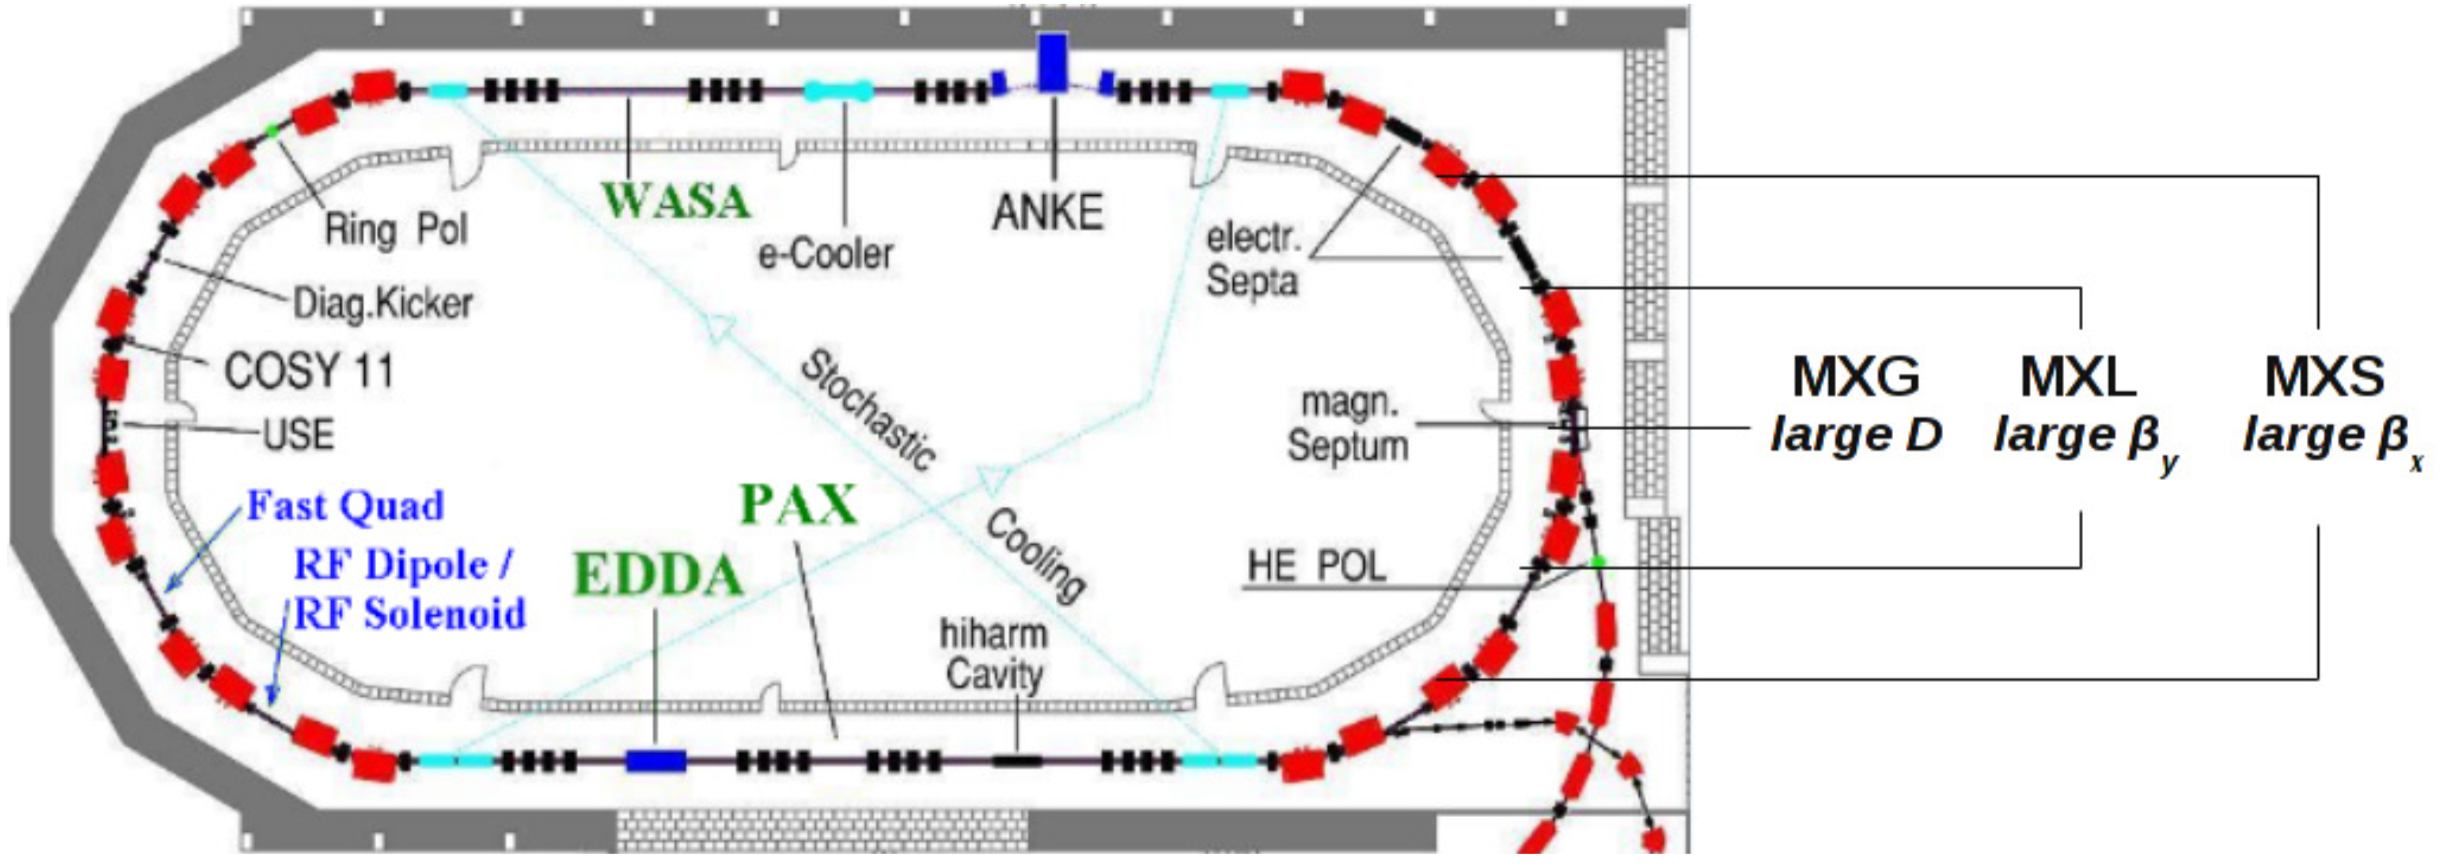
\includegraphics[width=\linewidth]{images/chapter4/COSY-sextupoles}
	\caption{COSY ring with marked sextupole positions. (Image taken from~\cite{Guidoboni:STORI14}.)}
\end{figure}

\subsection{Optimization procedure}
In this section we describe the optimization procedure using the example of the 2014 experiment.~\cite{Guidoboni:STORI14}
The SCT optimization experiment was first performed in 2012, but then only the MXS field strength was varied.
In 2014, a comprehensive (the field strengths of all three sextupole families were varied) SCT optimization
study was done for the first time.

To separate the effects related to the beam emittances and the 
second-order momentum dispersion $(\dpop)^2$, the beam was prepared in two different ways.

When studying the effect associated with a large $(\dpop)^2$, a polarized deuteron beam injected 
at $p=0.97$~GeV/c momentum is first cooled for 60 seconds, so that its emittance is minimized. 
After the cooling is turned off, the beam is bunched (harmonic number $h=1$). 
Bunching is required to minimize linear spin decoherence effects.

When studying the effect associated with horizontal emittance,~\footnote{Decoherence associated with 
	vertical emittance could not be studied because of acceptance limitations.} the beam is 
cooled and bunched simultaneously for the initial 60 seconds, after which cooling is turned off,
and horizontal heating is turned on for 5 seconds. The beam is heated by applying white noise to 
the horizontal kicker plates.

In both cases the polarization is vertically-oriented at injection. It is flipped by an RF solenoid 
after the beam preparation at the 80-th second.

Polarization is continuously measured by extracting the beam onto a 17 mm thick carbon target and
detecting the scattered deuterons at the EDDA polarimeter. 
Extraction is done by applying white noise to the vertical kicker. Elastic scattering of deuterons on 
carbon is a spin sensitive process with a large cross section.

The EDDA scintillators were grouped in four sectors (up, right, down, left); event rate asymmetry between the
left and right sectors is proportional to the beam's vertical polarization, the one between the up and down -- 
to the horizontal polarization component. Horizontal plane spin precession occurs at a a rate which greatly exceeds the polarimeter sampling rate, which is why a special data acquisition system was developed in 2012.~\cite{COSY:DAQ}

As a result of the experiment~\cite{Guidoboni:STORI14} a possibility of reaching an SCT over 1,000 seconds at COSY was shown. 

\subsection{SCT change when going from the external to the internal beam layers}
SCT optimization results obtained during the April-May 2019 beam time are shown below.

In the Figure series~\ref{fig:April2019:Polarization} the up-down cross section asymmetry measurement 
results are presented. In the first two figures one can observe that the rate of depolarization changes from
high in the first half (100 to 150 seconds) of the measurement cycle to significantly lower in the second half.
In Figure~\ref{fig:Polariation:recovery-from-halo-to-core} especially, we observe that polarization is increasing in the 130 to 150 second range, before it begins to gradually decrease again.
\begin{figure}[h]\centering
	\begin{subfigure}{\linewidth}
		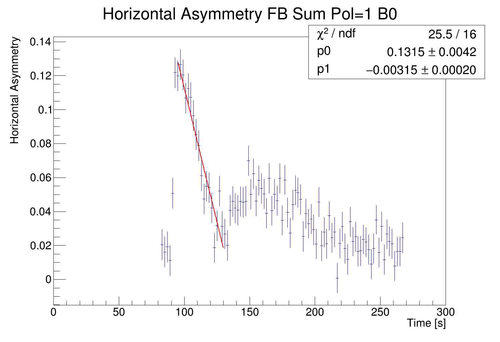
\includegraphics[height=.35\paperheight]{images/chapter4/SCT-April-2019/11th_19-55}
		\caption{SCT = $20.87 \pm 1.49$ sec.\label{fig:Polariation:recovery-from-halo-to-core}}
	\end{subfigure}
	\begin{subfigure}{\linewidth}
		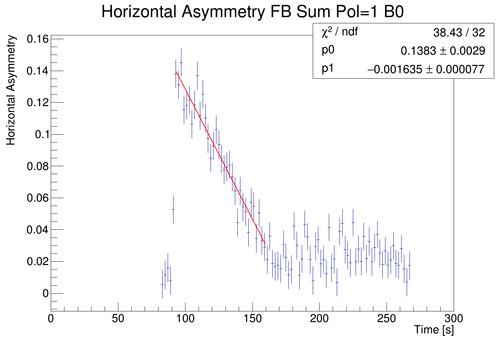
\includegraphics[height=.35\paperheight]{images/chapter4/SCT-April-2019/11th_20-20}
		\caption{SCT = $42.3 \pm 2.2$ sec.}
	\end{subfigure}
\end{figure}
\begin{figure}[h]\ContinuedFloat\centering
	\begin{subfigure}{\linewidth}
		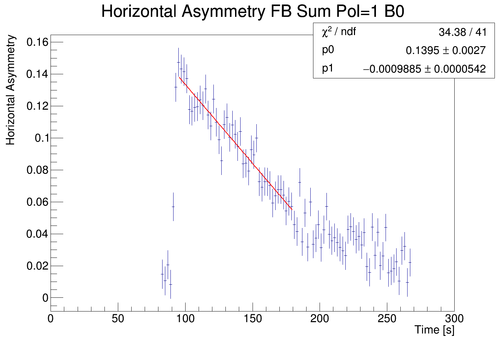
\includegraphics[height=.35\paperheight]{images/chapter4/SCT-April-2019/11th_20-31}
		\caption{SCT = $70.6 \pm 4.1$ sec.\label{fig:Polarization:halo-and-core-similar}}
	\end{subfigure}
	\begin{subfigure}{\linewidth}
		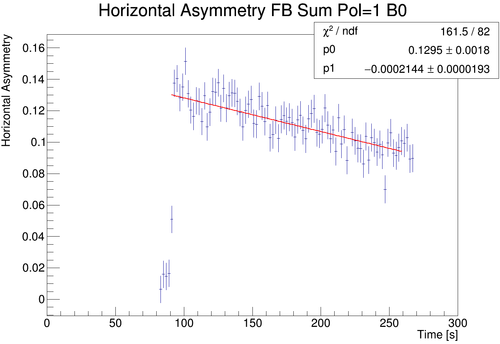
\includegraphics[height=.35\paperheight]{images/chapter4/SCT-April-2019/13th_03-23}
		\caption{SCT = $302.0 \pm 27.5$ sec.}
	\end{subfigure}
	\caption{Horizontal polarization measurements during SCT optimization during the axion search experiment done in April-May 2019.\label{fig:April2019:Polarization}}
\end{figure}

Such behavior can be explained by the non-uniformity of the polarization distribution. In the first half
of the measurement cycle particles from the outer (halo) beam layer are being sampled, while by the second half
those get exhausted, and the polarization of the internal (core) layer is being probed. Since the core is
more dense than the halo, the orbit length (hence spin tune) dispersion is less pronounced 
for its particles.

\subsection{SCT dependence on sextupole strength}
SCT dependence on the relative strengths of, respectively, the 
MXL and MXG sextupoles, measured during the April-May 2019 beamtime
is presented in Figure~\ref{fig:SCT_scan}. A resonance-type pattern can be observed.

\begin{figure}[h]\centering
	\begin{subfigure}{\linewidth}
		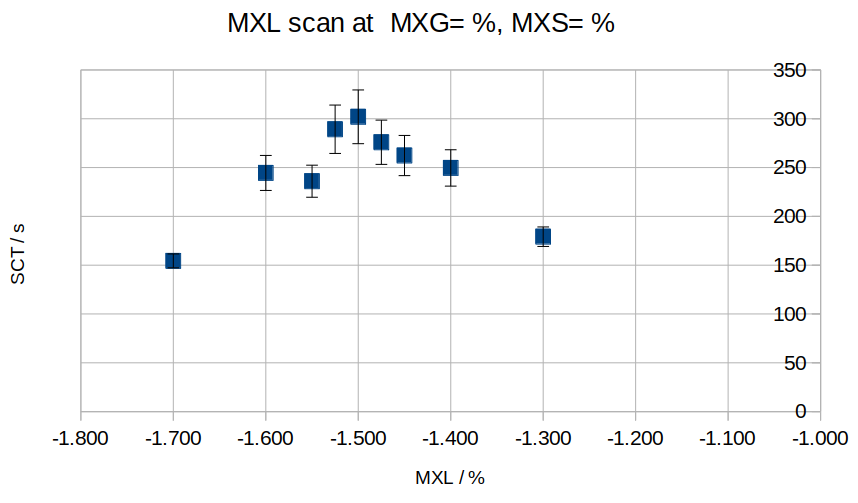
\includegraphics[height=.35\paperheight]{images/chapter4/SCT-April-2019/MXL_scan}
		\caption{MXL sextupole.}
	\end{subfigure}
	\begin{subfigure}{\linewidth}
		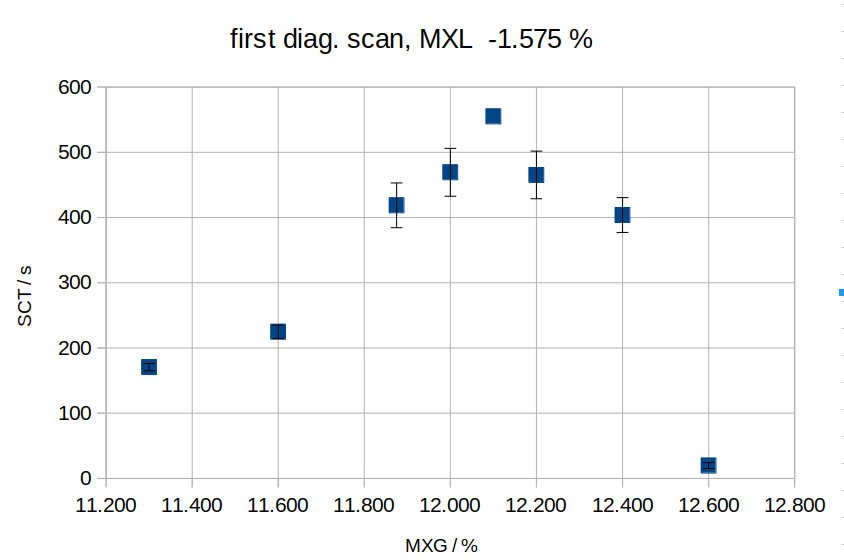
\includegraphics[width=.6\paperheight]{images/chapter4/SCT-April-2019/MXG_scan}
		\caption{MXG sextupole}
	\end{subfigure}
	\caption{SCT as a function fo the sextupole strength.\label{fig:SCT_scan}}
\end{figure}

Since COSY operates at an energy that is significantly far removed from spin resonance 
we decided to check if this pattern can be seen (within the framework of our numerical model) 
in the FS-type lattice. 
Spin tune standard deviation as a function of the corresponding sextupole gradient is plotted in Figure~\ref{fig:SCT_resonance}. 
(Data were taken from the simulation described in section~\ref{sec:decoh:sim-imperfect}.)
The same resonance pattern is observed as in the experiment.

\begin{figure}[h]
	\centering
	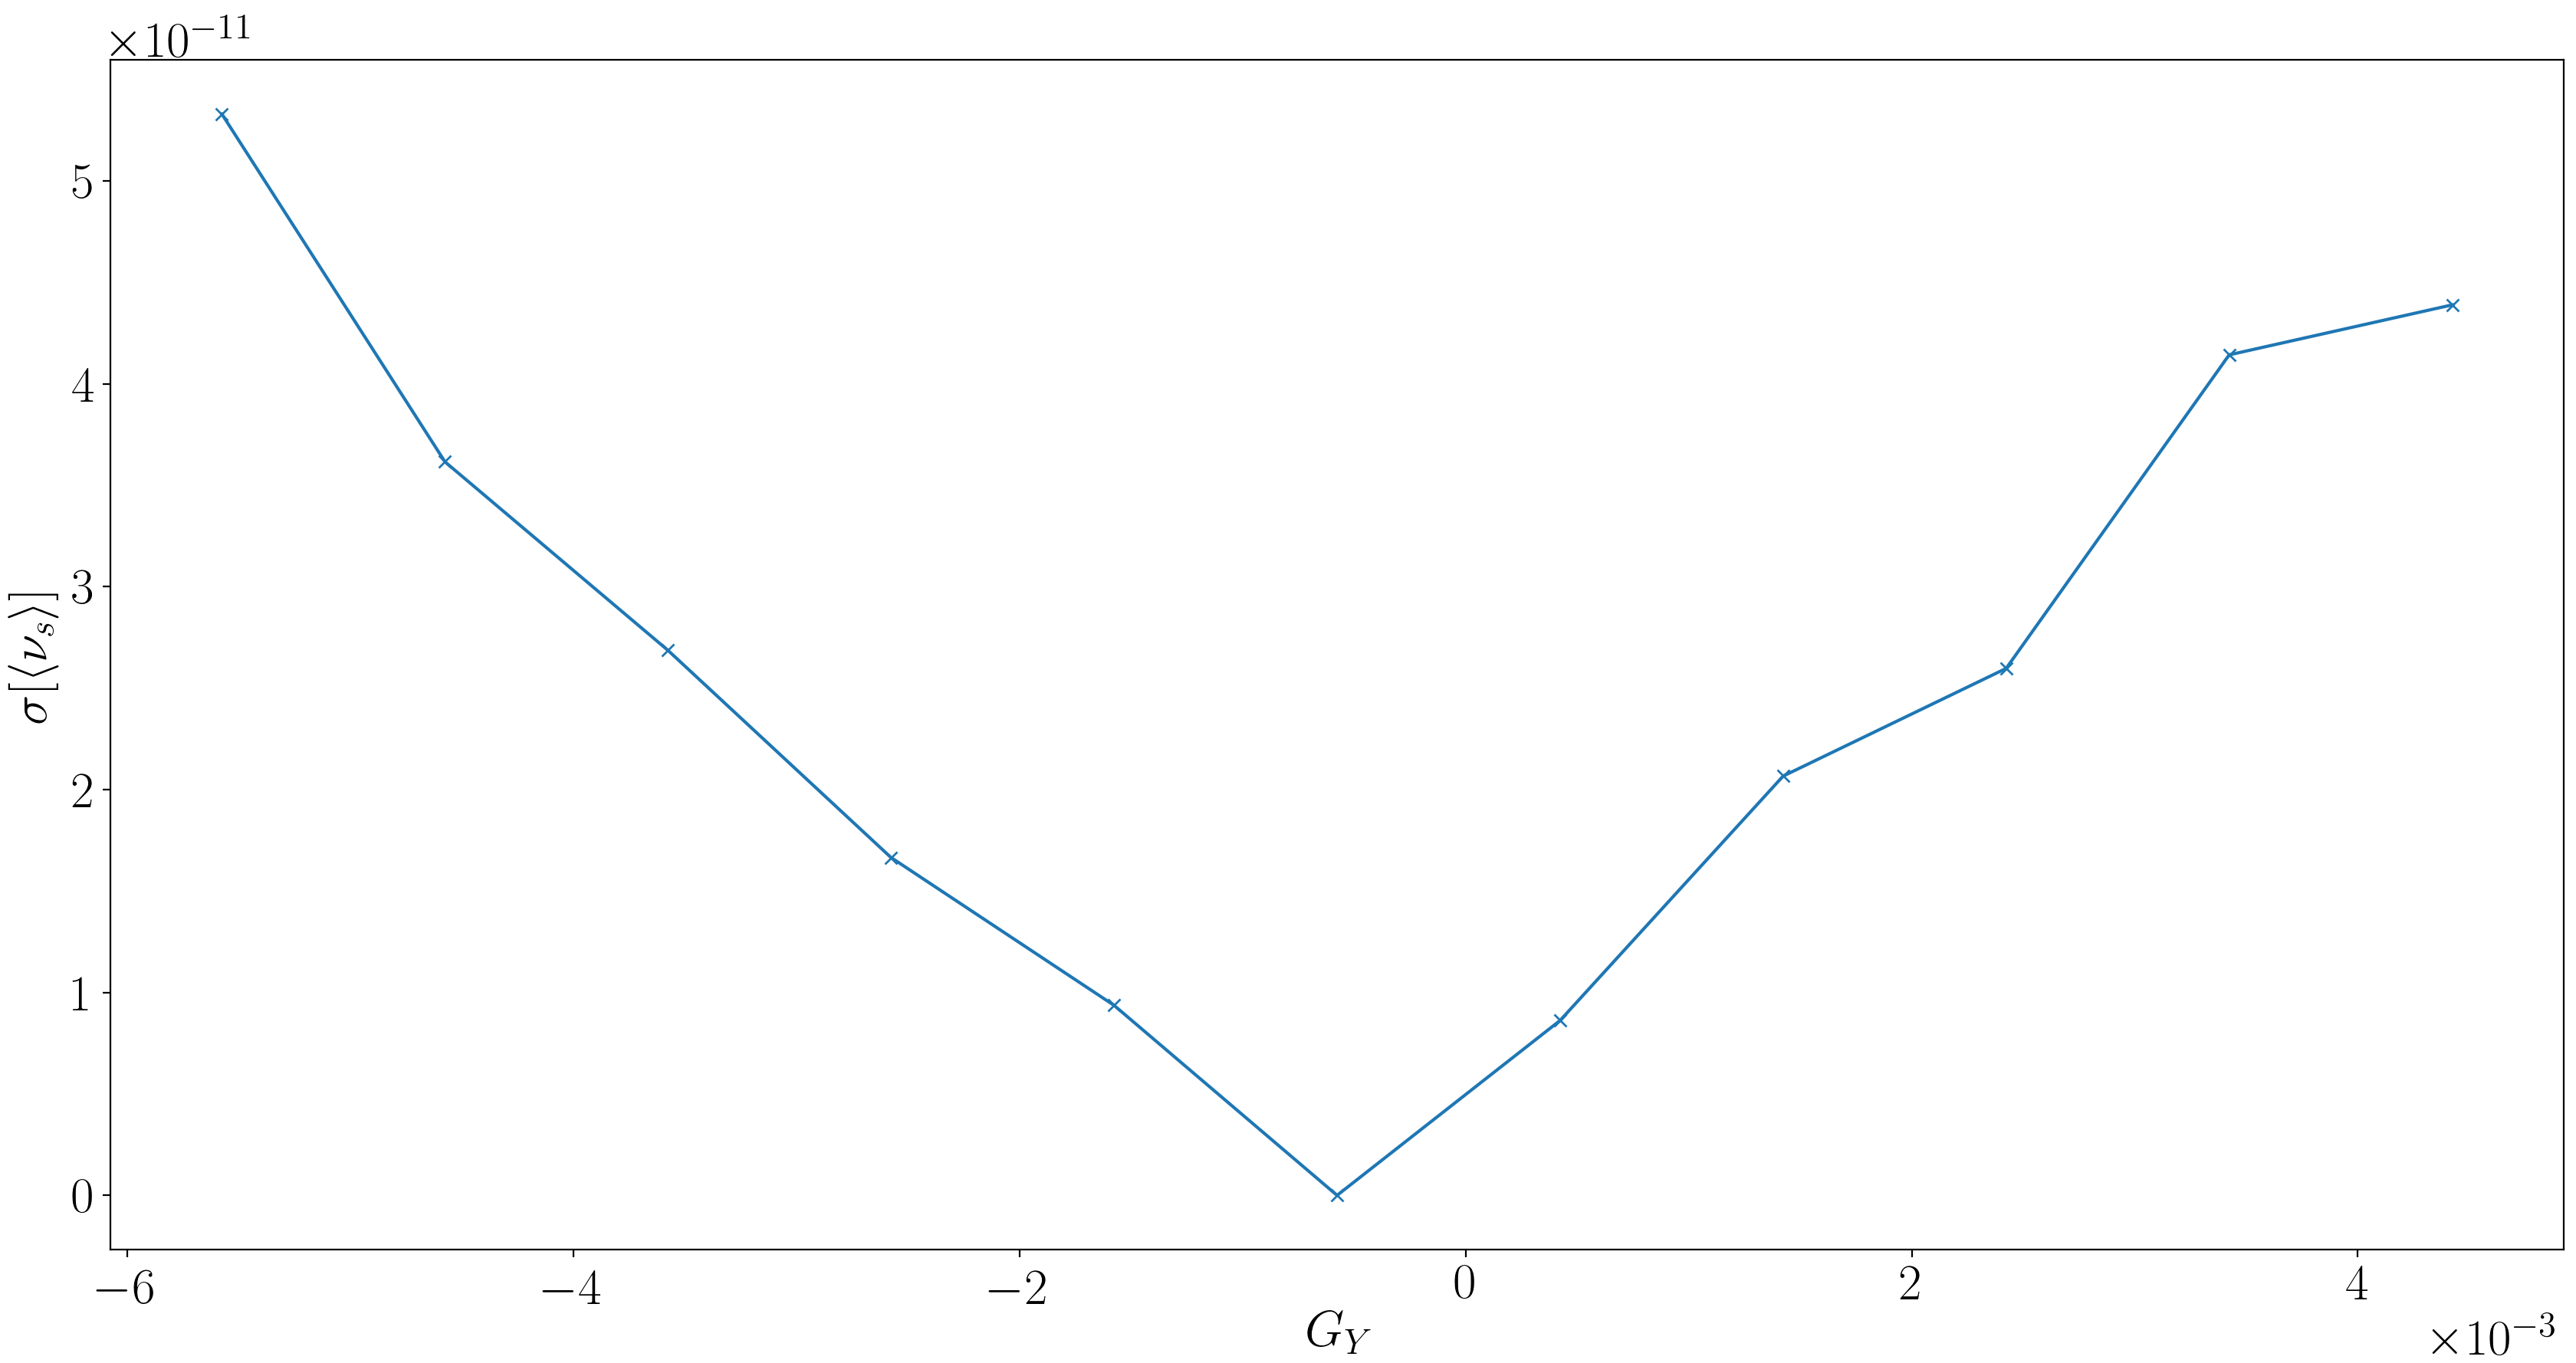
\includegraphics[width=\linewidth]{images/decoh_sim/stune_sd_vs_sext_strength_resonance}
	\caption{Spin tune dispersion as a function of the sextupole field gradient.\label{fig:SCT_resonance}}
\end{figure}



\clearpage
